\subsection{Структурно функциональная схема программного обеспечения}%, в состав которого входит разрабатываемый программный модуль с четкой формулировкой решаемых им задач}

Данное програмное обеспечение разрабатывается для задач оценки деформации твердого тела. Программное обеспечение состоит из нескольких блоков, представленных на рисунке \ref{pic:shema_PO}.

\begin{itemize}
\item ПО для оценки деформации ``Deformation Analysis''
\item Форма для ввода входных параметров ``strain\_calculate.qml''
\item ПО для расчета деформации твердого тела ``lucas\_kanade''
\end{itemize}

Программа ``Deformation Analysis'' разрабатывалась сотрудниками ИФПМ и служит средством для запуска и отображения выходных результатов. Форма ``strain\_calculate.qml'' является более удобным способом запуска основного приложения. 

\begin{figure}[ht]
\center{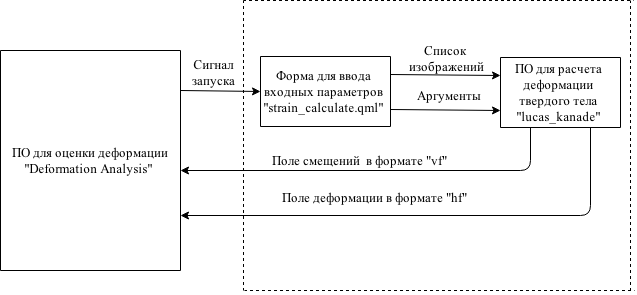
\includegraphics[width=0.8\linewidth]{shema_PO}}
\caption{Структура разработанного ПО}
\label{pic:shema_PO}
\end{figure}

\begin{figure}[ht]
\center{
\includegraphics[width=0.8\linewidth]{idef0}}
\caption{Функциональная схема}
\label{pic:idef0}
\end{figure}

\subsection{Характеристику входных и выходных информационных потоков разрабатываемого модуля}

\subsection{Сведения о платформе реализации с указанием основных функций операционной системы, необходимых для работы модуля}
\subsection{Обоснование целесообразности разработки оригинальных модулейпрограммного обеспечения}
\subsection{Обоснование выбора технологии программирования и средствразработки}
\subsection{Обоснование способа организации входных и выходных, промежуточных информационных потоков, использование оперативной и дисковойпамяти, кэширование данных}
\subsection{Учет эргономических критериев при разработке интерфейса пользователя}% (выбор цветовой палитры экранных форм, расположение элементовуправления на них, использование «горячих» клавиш  акселераторов, выпадающих меню и пр.)}
Интерфейс программы представлен в двух реализациях.
Первый - консольная программа в стиле классического Unix.

\begin{figure}[ht]
\center{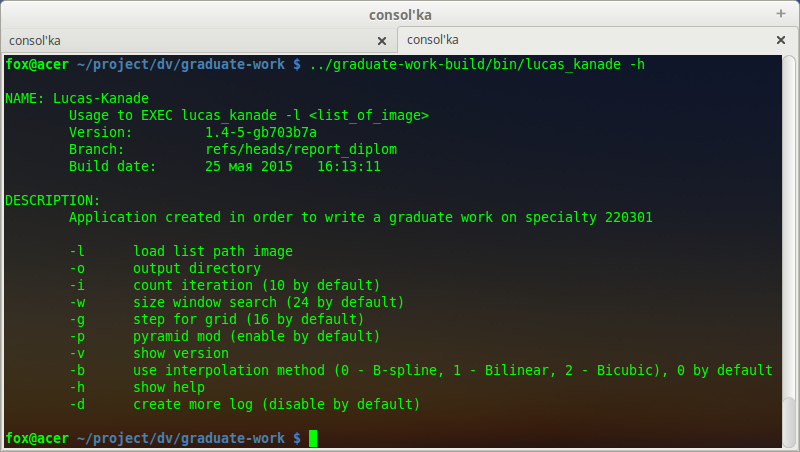
\includegraphics[width=0.8\linewidth]{consol_screen}}
\caption{Пример консольного интерфейса}
\label{pic:con_scr}
\end{figure}

Второй графический - более удобный для неопытного пользователя. 

\begin{figure}[ht]
\center{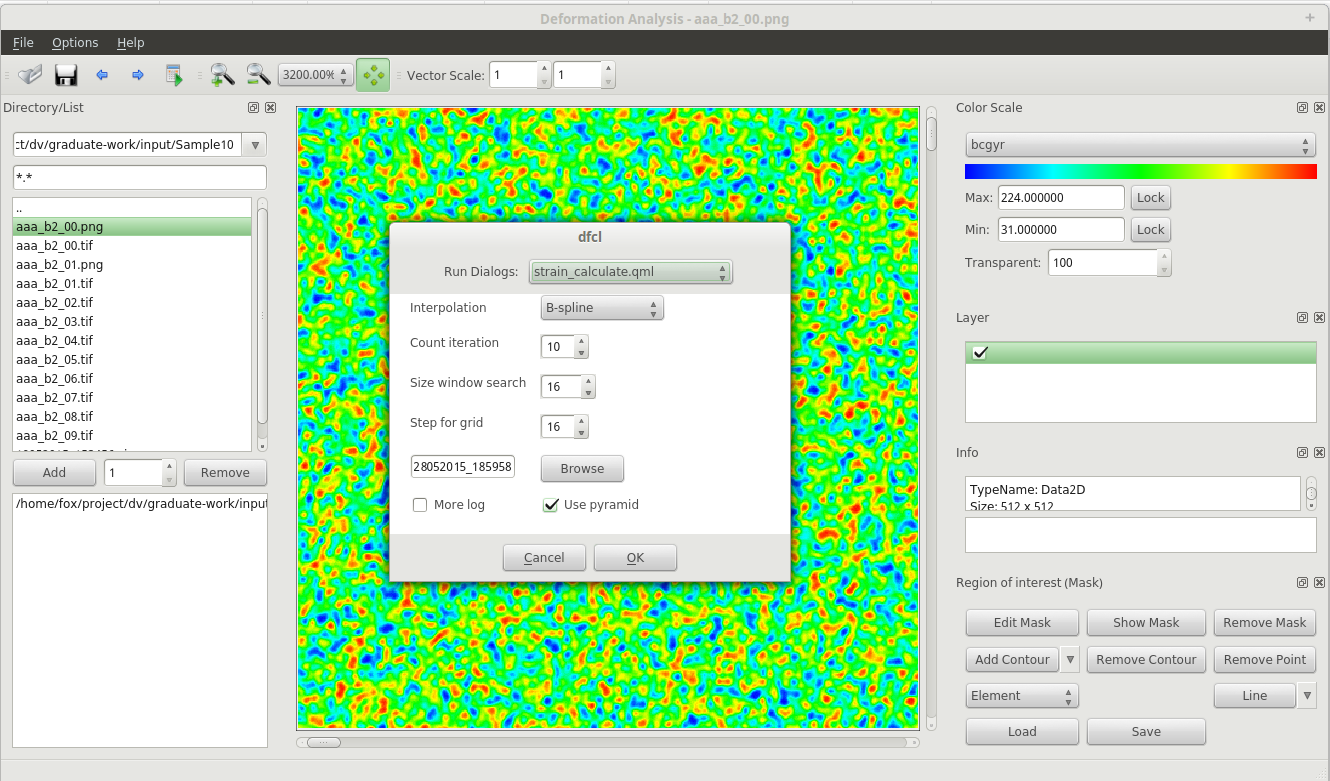
\includegraphics[width=0.6\linewidth]{gui_screen}}
\caption{Пример графического интерфейса}
\label{pic:gui_scr}
\end{figure}

\subsection{Справочную систему пользователя для разрабатываемого модуля,требования к уровню квалификации пользователя}
\subsection{Листинг программы с комментариями, поясняющими работу основных блоков}
\subsection{Блоксхему оригинальных, разработанных автором, алгоритмовработы основных, по мнению автора, программных модулей (1  3 блоксхемы,каждая не более, чем на 1 стр} формата А4)}
\subsection{Тестовый пример для контроля адекватного функционированияразработанного программного модуля и протокол (листинг) результатов работыпрограммы на этом тестовом примере}

Ориентировочный перечень иллюстрационно графического материала к дипломному проекту при разработке программного продукта:
\begin{enumerate}
\item  укрупненная структурно функциональная схема программного обеспечения, в составе которого работает разрабатываемый модуль. Разрабатываемый модуль должен быть визуально выделен на общей схеме (обведен штриховойрамкой, обозначен другим цветом и т.д.);
\item  структурно функциональная схема разрабатываемого программного модуля с обозначением входящих в него функциональных элементов и связеймежду ними. В связях надлежит доступными средствами выделить различные виды информационных потоков: символьные и кодовые массивы, бинарные сигналы индикации и управления, событийную информацию;
\item  основные математические соотношения в виде формул и выражений (при разработке вычислительных программ не более, чем 1 плакат формата А1);
\item  блоксхема алгоритма работы модуля с достаточной степенью детализации (при наличии в разработке оригинальных и неочевидных алгоритмических решений);
\item  изображения экранных форм в различных режимах работы программы(при разработке интерфейсных модулей);
\item  материал, иллюстрирующий работу программы на тестовом или реальном примере, с использованием графиков, таблиц и пр.
\end{enumerate}